\chapter{Results and Discussions}

\section{Dissecting XBot ransomware}

Xbot ransomware \cite{xbot} was mainly targeted in Russia or Australia.
As this statement can be proved, as we analysed many codes are commented in Russian language.

Reverse engineered the above app using dex2jar software.

\begin{figure}[H]
\centering
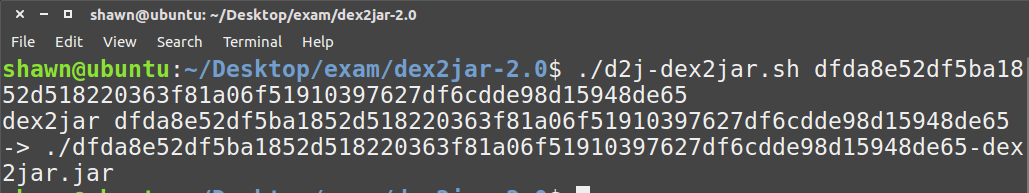
\includegraphics[scale=0.3]{dex2jar}
\caption{Using dex2jar on the xbot ransomware}
\label{fig:ra}
\end{figure}

The output is a jar file which can be opened in JD-GUI.
Using JD-GUI, the java files can be saved.

\begin{figure}[H]
\centering
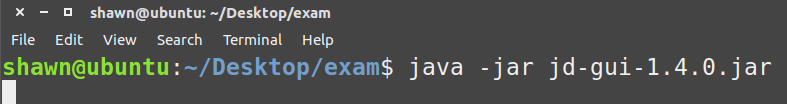
\includegraphics[scale=0.5]{jd-gui1}
\caption{Opening jar files using jd-gui}
\label{fig:ra}
\end{figure}

\begin{figure}[H]
\centering
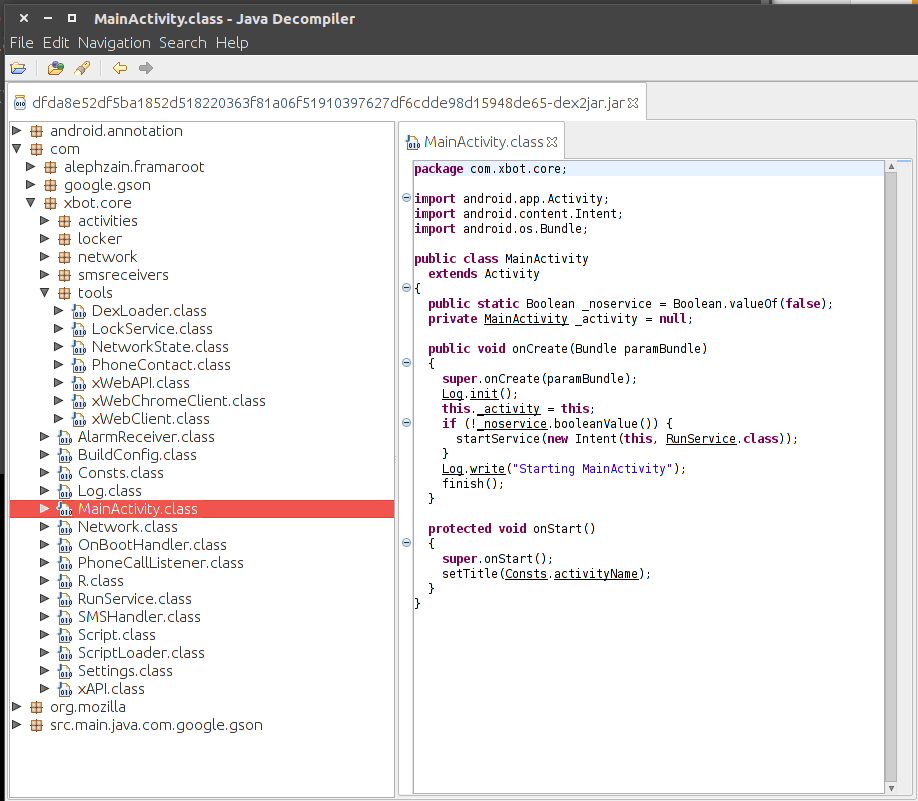
\includegraphics[scale=0.3]{jd-gui2}
\caption{jd-gui with all java files of xbot}
\label{fig:ra}
\end{figure}


After being installed on an Android device, Xbot contacts to the C2 server for further action.
Three of the actions was phising and one was activity hijacking.

\begin{figure}[H]
\centering
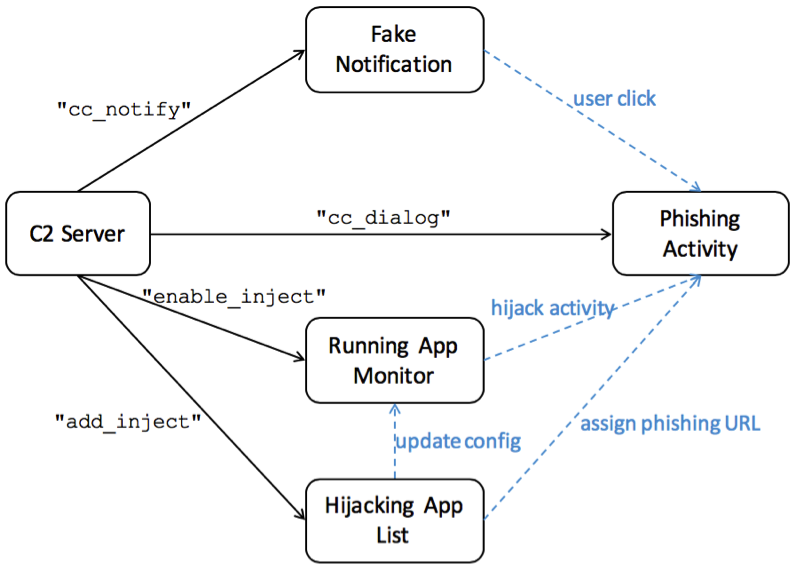
\includegraphics[scale=0.5]{xbot2}
\caption{Xbot's phising commands}
\label{fig:xbot2}
\end{figure}

When the C2 server gives a command of "cc\_notify", the app will display a notification based on ur location.
Which means if you are in Russia , then the notification will be in Russian language.
Rest of the world, it will be displayed in English.


\begin{figure}[H]
\centering
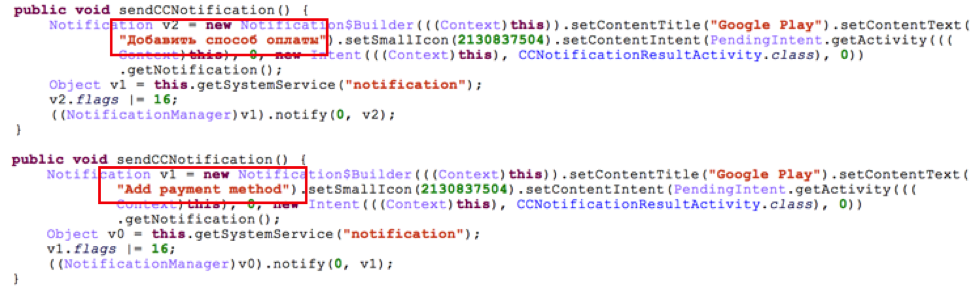
\includegraphics[scale=0.8]{xbot3}
\caption{Code for displaying the fake notification}
\label{fig:ra}
\end{figure}

Notification says that "add payment method" including the Google Play logo.
After clicking on the notification the user will be seeing a webpage in webview downloaded from the C2 server.
All the functionality is similar to the Google Play add payment method version.
All the information that the user gives will be saved to the C2 server.
The information saved are :-
\begin{itemize}
    \item credit card number
    \item expiration date
    \item CVV number
    \item card holder's name
    \item card holder's billing address
    \item card holder's phone number
    \item VBV (Verified by Visa) or McSec (MasterCard SecureCode) number
\end{itemize}

\begin{figure}[H]
\centering
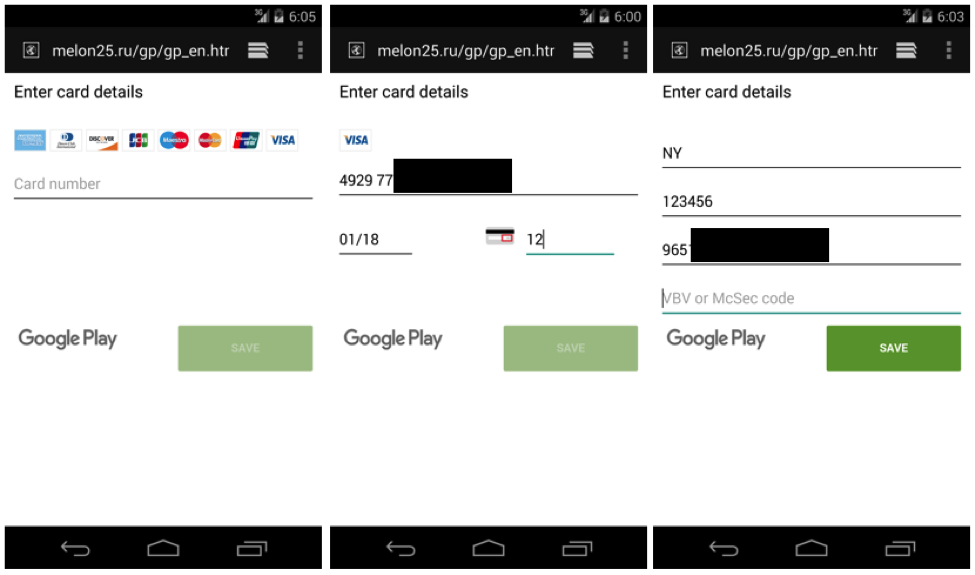
\includegraphics[scale=0.5]{xbot4}
\caption{Fake Google Play payment page}
\label{fig:ra}
\end{figure}

If the C2 command is "cc\_dialog", no notification will be displayed, the fake Google play add payment method page will be displayed.
If the C2 command is "enable\_inject", the app will check for all running apps using getRunningTasks() API in Android. 
They will search if there is any Google Play store app or one of the seven Australian app banks and immediately popup another activity on the top of the running app. 
This is called "activity hijacking".


\begin{figure}[H]
\centering
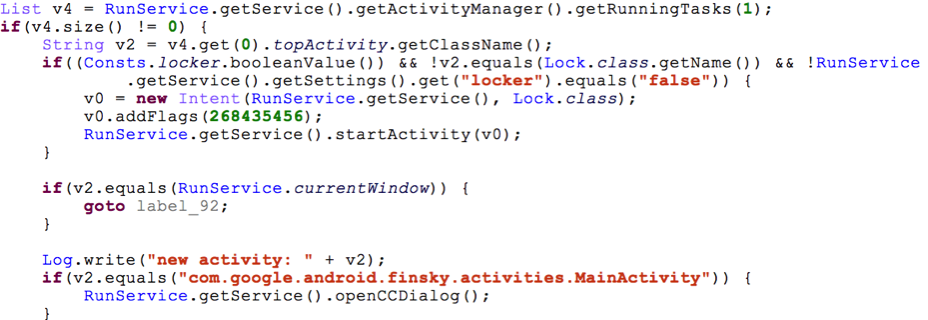
\includegraphics[scale=0.8]{xbot6}
\caption{Code for hijacking Google Play and banking apps}
\label{fig:ra}
\end{figure}

After installing xbot, it may ask for device administrator permissions.
If the C2 server sends "killon", the device will be set to silent mode and reset the password to "1811blabla".


\begin{figure}[H]
\centering
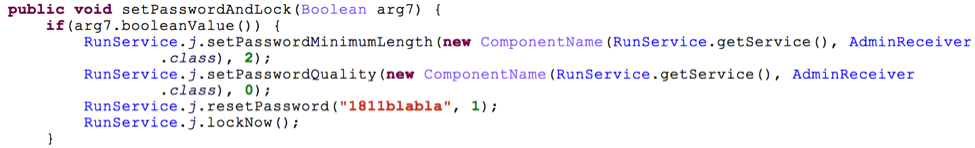
\includegraphics[scale=0.8]{xbot9}
\caption{Code to change the device password}
\label{fig:ra}
\end{figure}

If the C2 command is "enable\_locker", it will display the user that the phone is locked and files are encrypted.
The displayed thing is a webpage in webview from the address specified by the server.

\begin{figure}[H]
\centering
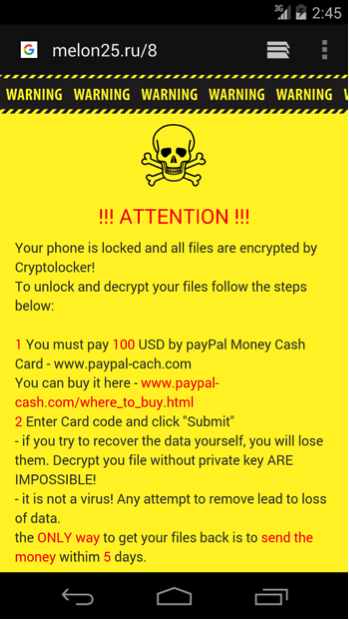
\includegraphics[scale=0.5]{xbot10}
\caption{Xbot ransom page}
\label{fig:ra}
\end{figure}

Xbot overrides onBackPressed(), onDestroy() and onPause() callback methods which makes the user to not get away from the page.
At the same time the xbot starts to encrypt the files in the external storage.
The encryption algorithm they used is XOR each byte of all files with an integer whose value is 50.

\begin{figure}[H]
\centering
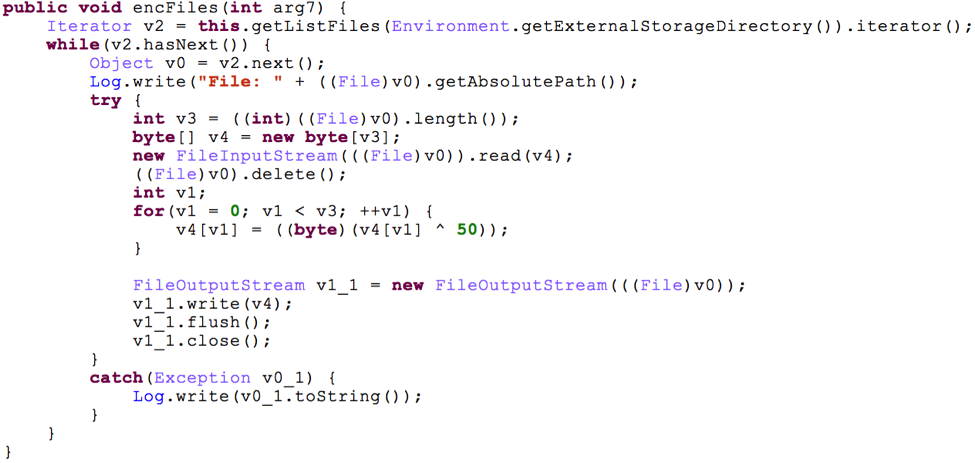
\includegraphics[scale=0.8]{xbot11}
\caption{Code to encrypt files in internal storage}
\label{fig:ra}
\end{figure}




\section{Detecting ransomwares using crowd sourcing App}

This section describes the working of Ransomware-CrowdSource app.
Source code of the app can be accessed at \href{https://github.com/jithin005/Ransomware-CrowdSource}{Ransomware-CrowdSource App}.
The main components of the Ransomware-CrowdSource app is 
\begin{itemize}
    \item Checker - is a broadcast reciever.
    \item Monitoring - is a service.
    \item Service - MyFirebaseMessagingService - is a service
    \item MainActivity - is an activity which acts as an interface to the user.
\end{itemize}

\subsection{Checker}

\par A broadcast receiver is a program that works on some broadcast message.
The broadcast message that checker will be looking for is \\
"android.intent.action.PACKAGE\_ADDED"
It keeps looking for any new app is installed.
If installed the app will be sent to the server along with the package name.



\subsection{Monitoring}

\par This is a service which keeps on getting the ip address that each app uses.
A service is similar to daemon in linux.
The ip address that it gets will saved to a flat file.
This flat files will be uploaded periodically, after successful sending the file will be deleted from the device.

\subsection{MyFirebaseMessagingService}

\par I used Firebase to communicate from the server to the device.
The Firebase creates an ID for each user, this will be saved in the database of the server.
This ID will be used to contact the registered devices.
If any malicious traffic or app is found it will send the message to delete the app with the app name.
Below is the image of the notification received by the user from the server if a malicious app is found. 

\begin{figure}[H]
\centering
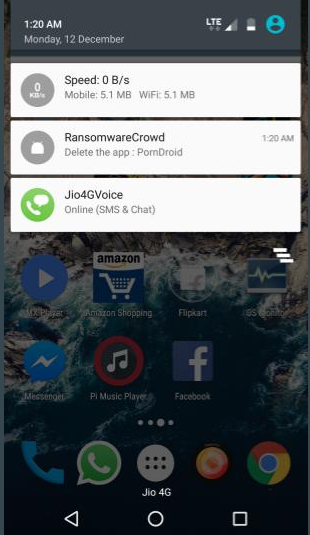
\includegraphics[scale=0.8]{notify}
\caption{Notification received by the registered device}
\label{fig:ra}
\end{figure}

\clearpage

\subsection{MainActivity}

\par This act as the user interface to the user.
This gives all the ip connections made by each app.
A screenshot of the MainActivity is shown below :-

\begin{figure}[H]
\centering
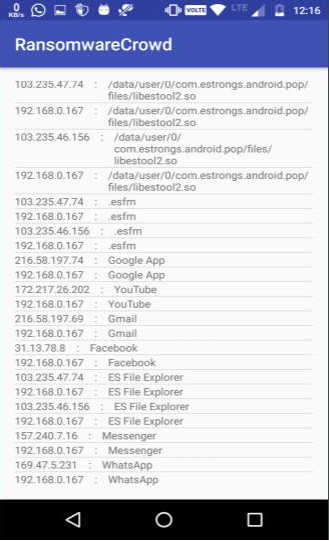
\includegraphics[scale=0.8]{front}
\caption{MainActivity with all app and its ip connections}
\label{fig:ra}
\end{figure}



